% ============================================================
% 第10章 射・有理写像・双有理幾何
% ============================================================
\chapter{射・有理写像・双有理幾何}
\label{ch:ch10}

\begin{chapterlead}
幾何学の対象を理解するには，対象そのものだけでなく「対象の間の写像」を理解しなければならない．
第5章ではアフィン多様体の間の正則写像を多項式写像として導入し，それが座標環の準同型と1対1に対応することを見た．
本章ではこれを射影多様体を含む一般の（準射影）多様体へと拡張する．
射影多様体の間の写像は大域的には多項式で書けないことがあり，「局所的に多項式の商で書ける」という定義が必要になる．
さらに，至るところで定義されているとは限らない\textbf{有理写像}を導入し，「稠密な開集合上で同型」という緩い同値関係（双有理同値）で多様体を分類する双有理幾何の考え方を学ぶ．
最後に，これらの対応を圏と関手の言葉で整理する．
\end{chapterlead}

% ------------------------------------------------------------
\section{多様体間の射}
% ------------------------------------------------------------

\subsection{多様体の射の定義}

本章で扱う多様体は次のクラスである．

\begin{mydef}{準射影多様体}{ch10-quasiproj}
射影多様体 $\overline X\subset\PP^n$ の空でない Zariski 開集合 $X\subset\overline X$ を\textbf{準射影多様体}という．
アフィン多様体（$\A^n=U_0\subset\PP^n$ の閉部分多様体）と射影多様体はいずれも準射影多様体である．
\end{mydef}

まず「関数」を定める．射影空間上では同次多項式そのものは関数にならない（$F(\lambda x)=\lambda^dF(x)$）が，同じ次数の同次多項式の商は値が定まる．

\begin{mydef}{正則関数}{ch10-regfun}
$X$ を準射影多様体，$U\subset X$ を開集合とする．関数 $f:U\to k$ が点 $p\in U$ で\textbf{正則}であるとは，$p$ の開近傍 $V\subset U$ と，同じ次数の同次多項式 $G,H$ で $H$ が $V$ 上で消えないものが存在して
\[
  f(q)=\frac{G(q)}{H(q)}\qquad(q\in V)
\]
となることをいう．$U$ の各点で正則な関数を $U$ 上の正則関数といい，その全体を $\OO_X(U)$ と書く．
\end{mydef}

アフィン多様体 $X$ では，大域的な正則関数は多項式関数に一致する：$\OO_X(X)=k[X]$（第5章・第6章）．
局所的な表示 $G/H$ は一般に点ごとに取り替える必要がある．これが次の層の考え方（第11章）につながる．

\begin{mydef}{射}{ch10-morphism}
準射影多様体の間の写像 $\varphi:X\to Y$ が\textbf{射}（morphism, 正則写像）であるとは，
\begin{enumerate}
  \item $\varphi$ は Zariski 位相について連続であり，
  \item 任意の開集合 $V\subset Y$ と $f\in\OO_Y(V)$ に対し，$\varphi^*f=f\circ\varphi\in\OO_X(\varphi^{-1}(V))$ である
\end{enumerate}
ことをいう．すなわち「正則関数を引き戻すと正則関数になる」連続写像である．
\end{mydef}

$Y\subset\PP^m$ のときは，次の同値な言い換えが実用的である．

\begin{myprop}{射の局所表示}{ch10-localform}
写像 $\varphi:X\to Y\subset\PP^m$ が射であるための必要十分条件は，各点 $p\in X$ に対し，$p$ の開近傍 $V$ と\emph{同じ次数}の同次多項式 $F_0,\dots,F_m$ で，$V$ 上で同時には消えないものが存在して
\[
  \varphi(q)=[F_0(q):\dots:F_m(q)]\qquad(q\in V)
\]
と書けることである．
\end{myprop}

\begin{proof}[証明の概略]
十分性：$\varphi(p)\in U_j=\{y_j\neq0\}$ なら，$p$ の近くで $F_j\neq0$ であり，$U_j\cong\A^m$ の座標 $y_i/y_j$ を引き戻すと $F_i/F_j$ となって正則．$U_j$ 上の正則関数は局所的に $y_i/y_j$ の多項式の商なので，引き戻しも正則である．
必要性：$\varphi^*(y_i/y_j)$ は $p$ の近傍で $G_i/H_i$ と書けるので，通分して共通の分母をはらえばよい．
\end{proof}

\begin{myex}{Veronese 写像}{ch10-veronese}
$v_2:\PP^1\to\PP^2$，$[s:t]\mapsto[s^2:st:t^2]$ は射である（$s^2,t^2$ は同時に消えない）．
像は円錐曲線 $Q=\Zero(xz-y^2)$ である．
\end{myex}

\begin{myex}{局所的にしか書けない射}{ch10-conicproj}
円錐曲線 $Q=\Zero(xz-y^2)\subset\PP^2$ から $\PP^1$ への写像を
\[
  \psi([x:y:z])=\begin{cases}[x:y] & (x,y)\neq(0,0)\\ [y:z] & (y,z)\neq(0,0)\end{cases}
\]
で定める．$Q$ 上では $xz=y^2$ なので，両方が定義される点では $[x:y]=[y:z]$（$xz=y^2$ より $x:y=y:z$）であり，well-defined である．
$Q$ のすべての点で少なくとも一方が定義されている（$x=y=0$ なら $z\neq0$）ので $\psi$ は射であり，$v_2$ の逆写像になっている．
しかし $\psi$ を1組の同次多項式で大域的に表すことはできない．
このように，射の定義が「局所的に」でなければならないことは射影多様体では本質的である．
\end{myex}

\subsection{射の合成}

\begin{myprop}{合成}{ch10-composition}
$\varphi:X\to Y$, $\psi:Y\to Z$ が射ならば，合成 $\psi\circ\varphi:X\to Z$ も射である．
\end{myprop}

\begin{proof}
連続写像の合成は連続．$f\in\OO_Z(W)$ について $(\psi\circ\varphi)^*f=\varphi^*(\psi^*f)$ であり，$\psi^*f\in\OO_Y(\psi^{-1}W)$，さらに $\varphi^*(\psi^*f)\in\OO_X(\varphi^{-1}\psi^{-1}W)$．
\end{proof}

引き戻しは順序を反転させる：$(\psi\circ\varphi)^*=\varphi^*\circ\psi^*$．この\textbf{反変性}は10.5節で圏論的に整理する．

\begin{myex}{射の合成}{ch10-compex}
$v_2:\PP^1\to\PP^2$ と，射影変換 $T:\PP^2\to\PP^2$，$[x:y:z]\mapsto[x+z:2y:z-x]$ の合成は
\[
  T\circ v_2([s:t])=[s^2+t^2:2st:t^2-s^2]
\]
であり，$(s^2+t^2)^2=(2st)^2+(t^2-s^2)^2$ より，その像は円錐曲線 $\Zero(Y^2+Z^2-X^2)$（同次座標 $[X:Y:Z]$）である．
これは 10.3節で扱う「円の有理パラメータ表示」の射影版である．
\end{myex}

\subsection{恒等射}

各多様体 $X$ に対し，恒等写像 $\mathrm{id}_X:X\to X$ は射である（$\mathrm{id}_X^*f=f$）．
また射の合成は結合的であり，$\varphi\circ\mathrm{id}_X=\varphi=\mathrm{id}_Y\circ\varphi$ を満たす．
すなわち，準射影多様体と射は\textbf{圏}をなす（10.5節）．

\begin{myex}{包含写像・定値写像}{ch10-inclusion}
\begin{enumerate}
  \item 開部分多様体・閉部分多様体の包含写像 $Z\hookrightarrow X$ は射である．
  \item 1点への写像 $X\to\{pt\}$，および1点 $q$ への定値写像 $X\to Y$ は射である．
  \item 標準アフィン開集合の同一視 $\A^n\to U_0\subset\PP^n$，$(a_1,\dots,a_n)\mapsto[1:a_1:\dots:a_n]$ は射であり，その逆 $[x_0:\dots:x_n]\mapsto(x_1/x_0,\dots,x_n/x_0)$ も射である．
\end{enumerate}
\end{myex}

\subsection{同型}

\begin{mydef}{同型}{ch10-iso}
射 $\varphi:X\to Y$ に対し，射 $\psi:Y\to X$ で $\psi\circ\varphi=\mathrm{id}_X$，$\varphi\circ\psi=\mathrm{id}_Y$ となるものが存在するとき，$\varphi$ を\textbf{同型}といい，$X\cong Y$ と書く．
\end{mydef}

例\ref{ex:ch10-conicproj}により，非退化円錐曲線は $\PP^1$ と同型である．
重要なのは，\emph{全単射な射は同型とは限らない}ことである．

\begin{myex}{尖点曲線への全単射}{ch10-cuspbij}
$C=\Zero(y^2-x^3)\subset\A^2$ とし，$\nu:\A^1\to C$，$t\mapsto(t^2,t^3)$ を考える．
$\nu$ は全単射である（逆写像は $(x,y)\mapsto y/x$（$x\neq0$），$(0,0)\mapsto0$）．
しかし逆写像は射ではない．実際，座標環の準同型
\[
  \nu^*:k[C]=k[x,y]/(y^2-x^3)\to k[t],\qquad x\mapsto t^2,\ y\mapsto t^3
\]
の像は $k[t^2,t^3]$ であり，$t$ を含まない．もし $\nu$ が同型なら $\nu^*$ は同型でなければならない（第5章）．
幾何学的には，$C$ は原点で特異（第7章）だが $\A^1$ は滑らかなので，同型にはなりえない．
\end{myex}

\begin{myex}{Frobenius 写像}{ch10-frobenius}
$\mathrm{char}\,k=p>0$ のとき，$F:\A^1\to\A^1$，$t\mapsto t^p$ は全単射な射だが，$F^*:k[t]\to k[t]$，$t\mapsto t^p$ は全射でないので同型ではない．
\end{myex}

\begin{physbox}[同型と物理的同値]
物理では，2つの理論の「配位空間」が同じかどうかを問うとき，点集合として1対1であるだけでは不十分で，その上の「関数（観測量）」まで対応していなければならない．
尖点曲線の例では，点集合は $\A^1$ と1対1だが，観測量の代数 $k[t^2,t^3]$ は $k[t]$ より小さい：$t$ という「なめらかな座標」が観測量として存在しない．
代数幾何の同型の定義は「点と観測量の両方の同一視」を要求しており，量子論で状態空間と演算子代数の両方を比べるのと同じ精神である．
\end{physbox}

\subsection{射の基本性質}

\begin{myprop}{射の基本性質}{ch10-morprop}
\begin{enumerate}
  \item 射は Zariski 位相について連続であり，既約集合の像は既約である．
  \item アフィン多様体 $Y$ への射 $X\to Y\subset\A^m$ は，$m$ 個の正則関数 $f_1,\dots,f_m\in\OO_X(X)$ の組と同じである．
  \item （射影多様体の像は閉）$X$ が射影多様体ならば，任意の射 $\varphi:X\to Y$ の像 $\varphi(X)$ は $Y$ の閉集合である．
  \item $X$ が射影多様体ならば $\OO_X(X)=k$，すなわち大域的な正則関数は定数のみである．
\end{enumerate}
\end{myprop}

\begin{proof}[証明の概略]
(1)：既約集合 $Z$ の像が $A\cup B$（閉集合）に含まれれば $Z\subset\varphi^{-1}(A)\cup\varphi^{-1}(B)$．
(2)：命題\ref{prop:ch10-localform}のアフィン版．
(3)：射影空間の「完備性」と呼ばれる性質であり，消去理論の主定理（同次多項式系の共通零点の存在条件が係数の多項式で書けること）から従う．詳細は省略する．
(4)：$f\in\OO_X(X)$ は射 $f:X\to\A^1\subset\PP^1$ を定める．(3) より $f(X)$ は $\PP^1$ の既約閉集合で，$\infty$ を含まないから $\PP^1$ 全体ではない．したがって1点である．
\end{proof}

(4) は複素解析における Liouville の定理（コンパクト複素多様体上の正則関数は定数）の代数版である．射影空間が「コンパクト」であることの代数的な反映といえる．

第9章の射影次元定理を使うと，次の印象的な結果が得られる．

\begin{mycor}{次元を下げる射は定数}{ch10-PnPm}
$n>m$ ならば，任意の射 $\varphi:\PP^n\to\PP^m$ は定値写像である．
\end{mycor}

\begin{proof}[証明の概略]
$\PP^n$ からの射は大域的に同じ次数 $d$ の同次多項式 $F_0,\dots,F_m$（共通零点なし）で表されることが知られている（直線束の言葉では $\Pic\PP^n\cong\Z$，すなわち $\PP^n$ 上の直線束が $\OO(d)$ に限られることによる；$\OO(d)$ については第14章参照）．
$d\ge1$ とすると，$m+1\le n$ 個の超曲面 $\Zero(F_i)$ の交わりは第9章の射影次元定理により次元 $\ge n-(m+1)\ge0$ で，空でない．これは $F_i$ が共通零点を持たないことに反する．よって $d=0$，すなわち $\varphi$ は定数．
\end{proof}

\exprob{prob:ch10-1}
$\varphi:\PP^1\to\PP^3$，$[s:t]\mapsto[s^3:s^2t:st^2:t^3]$ がその像 $T$（ねじれ3次曲線）への同型であることを，逆写像を局所的に書き下すことにより示せ．

\exprob{prob:ch10-2}
$\A^1\setminus\{0\}$ と双曲線 $H=\Zero(xy-1)\subset\A^2$ が同型であることを示せ．
また $\A^1\setminus\{0\}$ は $\A^1$ と同型でないことを，大域的正則関数の環を比較して示せ．

% ------------------------------------------------------------
\section{有理写像}
% ------------------------------------------------------------

\subsection{有理写像の定義}

射影多様体の間の自然な写像には，いくつかの点で定義できないものが多い．
例えば $[x:y:z]\mapsto[x:y]$ は $x=y=0$ となる点 $[0:0:1]$ で意味を持たない．
こうした「ほとんど至るところで定義された写像」を扱うのが有理写像である．

\begin{mydef}{有理写像}{ch10-rational}
$X,Y$ を多様体とする．組 $(U,\varphi_U)$（$U\subset X$ は空でない開集合，$\varphi_U:U\to Y$ は射）を考え，
\[
  (U,\varphi_U)\sim(V,\varphi_V)\iff \varphi_U=\varphi_V\ \text{on}\ U\cap V
\]
で同値関係を入れる．その同値類を $X$ から $Y$ への\textbf{有理写像}といい，$\varphi:X\dashrightarrow Y$ と書く．
像が $Y$ で稠密なとき，$\varphi$ は\textbf{支配的}（dominant）であるという．
\end{mydef}

関係 $\sim$ が推移的であることは，「2つの射が稠密な開集合上で一致すれば共通の定義域全体で一致する」ことによる．
これは射の一致する点の集合が閉集合であり，既約な多様体では空でない開集合が稠密であることから従う．
すなわち多様体の間の射は，稠密な開集合上の値で決まってしまう．これは解析接続の一意性の代数版である．

$Y\subset\PP^m$ のときは，有理写像は同じ次数の同次多項式の組
\[
  \varphi=[F_0:\dots:F_m]
\]
（すべてが $X$ 上で恒等的には消えない）で与えられる．
共通因子 $H$ で割った $[F_0/H:\dots:F_m/H]$ も同じ有理写像を表す．

\subsection{定義域}

\begin{mydef}{定義域・不確定点}{ch10-domain}
有理写像 $\varphi:X\dashrightarrow Y$ の代表 $(U,\varphi_U)$ の $U$ 全体の和集合を $\varphi$ の\textbf{定義域} $\mathrm{dom}(\varphi)$ という．
これは $X$ の空でない開集合であり，$\varphi$ はその上の射として一意に定まる．
$X\setminus\mathrm{dom}(\varphi)$ の点を\textbf{不確定点}（indeterminacy point）という．
\end{mydef}

点 $p$ が定義域に入るかどうかを判定するには，表示 $[F_0:\dots:F_m]$ を（共通因子を割る，$X$ の方程式を使って書き換えるなどして）取り替え，$p$ で全部が同時に消えないものを見つければよい．

\begin{myex}{点からの射影}{ch10-projection}
$\pi:\PP^2\dashrightarrow\PP^1$，$[x:y:z]\mapsto[x:y]$ は点 $O=[0:0:1]$ からの射影である．
幾何学的には，点 $p\neq O$ に対し，$O$ と $p$ を結ぶ直線を $O$ を通る直線全体 $\cong\PP^1$ の元とみなす写像である．
$\mathrm{dom}(\pi)=\PP^2\setminus\{O\}$ であり，$O$ は不確定点である：$O$ に近づく方向によって $\pi$ の値の極限がすべての $[a:b]\in\PP^1$ をとりうるからである（$[ta:tb:1]\to O$ のとき $\pi=[a:b]$）．
\end{myex}

\begin{figure}[htbp]
\centering
\begin{tikzpicture}[scale=0.9]
  \fill (0,0) circle (2.2pt) node[below left] {$O=[0:0:1]$};
  \foreach \a in {10,35,60,85,110,135,160}
    \draw[gray] ({-0.6*cos(\a)},{-0.6*sin(\a)})--({3*cos(\a)},{3*sin(\a)});
  \draw[thick,blue] (-3,2.4)--(3.9,2.4) node[right] {$\PP^1$（直線 $z=0$ 方向の「行き先」）};
  \fill[red] ({1.2*cos(35)},{1.2*sin(35)}) circle (2pt) node[right] {$p$};
  \fill[blue] ({2.4/tan(35)},2.4) circle (2pt) node[above] {$\pi(p)$};
  \draw[thick,red,dashed] (0,0)--({2.4/tan(35)},2.4);
\end{tikzpicture}
\caption{点 $O$ からの射影 $\pi:\PP^2\dashrightarrow\PP^1$．各点 $p\neq O$ は $O$ を通る直線（$\PP^1$ の点）に送られる．$O$ 自身はすべての直線に乗っているため値が定まらない．}
\label{fig:ch10-projection}
\end{figure}

\begin{myex}{見かけの不確定点}{ch10-fake}
円錐曲線 $Q=\Zero(xz-y^2)$ に $\pi$ を制限すると，$[x:y]$ は $Q$ 上の点 $O=[0:0:1]\in Q$ で消える．
しかし例\ref{ex:ch10-conicproj}のように $Q$ 上では $[x:y]=[y:z]$ と書き換えられ，$O$ では $[y:z]=[0:1]$ と定義される．
すなわち $\pi|_Q:Q\dashrightarrow\PP^1$ は実際には射であり，$O$ は見かけ上の不確定点にすぎない．
幾何学的には，$O$ での値は「$O$ における $Q$ の接線」の方向である．
\end{myex}

\begin{myex}{標準 Cremona 変換}{ch10-cremona}
\[
  \sigma:\PP^2\dashrightarrow\PP^2,\qquad [x:y:z]\mapsto[yz:xz:xy]
\]
を\textbf{標準 Cremona 変換}という．$xyz\neq0$ では $[yz:xz:xy]=[1/x:1/y:1/z]$ である．
\begin{itemize}
  \item \textbf{不確定点}：3つの2次式が同時に消えるのは2つの座標が0のとき，すなわち $P_1=[1:0:0]$, $P_2=[0:1:0]$, $P_3=[0:0:1]$．
  これらでは表示をどう取り替えても定義できない（$P_3$ に直線 $y=tx$ に沿って近づくと $[tx\cdot z:xz:tx^2]\to[t:1:0]$ となり，$t$ に依存する）．
  \item \textbf{直線のつぶれ}：直線 $\{x=0\}$ 上（$P_2,P_3$ 以外）では $\sigma=[yz:0:0]=[1:0:0]=P_1$．すなわち座標三角形の各辺が対頂点に潰される．
  \item \textbf{対合性}：$\sigma\circ\sigma[x:y:z]=[x^2yz:xy^2z:xyz^2]=[x:y:z]$（$xyz\neq0$ で）．よって $\sigma$ は自分自身の逆である．
\end{itemize}
\end{myex}

\begin{figure}[htbp]
\centering
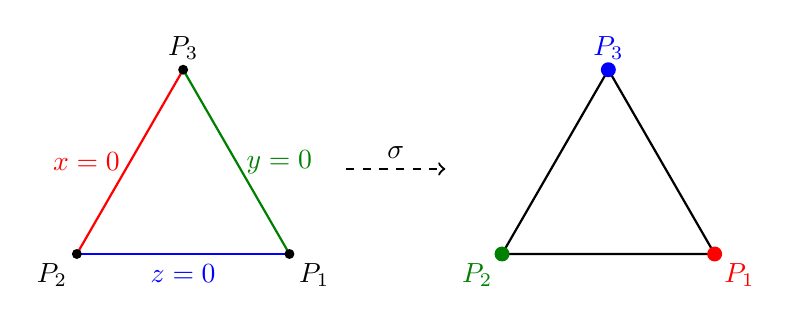
\begin{tikzpicture}[scale=0.9]
  \coordinate (A) at (0,0); \coordinate (B) at (3,0); \coordinate (C) at (1.5,2.6);
  \draw[thick,blue] (A)--(B) node[midway,below] {$z=0$};
  \draw[thick,green!50!black] (B)--(C) node[midway,right] {$y=0$};
  \draw[thick,red] (C)--(A) node[midway,left] {$x=0$};
  \fill (A) circle (2pt) node[below left] {$P_2$};
  \fill (B) circle (2pt) node[below right] {$P_1$};
  \fill (C) circle (2pt) node[above] {$P_3$};
  \draw[->,thick,dashed] (3.8,1.2)--(5.2,1.2) node[midway,above] {$\sigma$};
  \begin{scope}[xshift=6cm]
    \coordinate (A2) at (0,0); \coordinate (B2) at (3,0); \coordinate (C2) at (1.5,2.6);
    \draw[thick] (A2)--(B2)--(C2)--cycle;
    \fill[blue] (C2) circle (3pt) node[above] {$P_3$};
    \fill[red] (B2) circle (3pt) node[below right] {$P_1$};
    \fill[green!50!black] (A2) circle (3pt) node[below left] {$P_2$};
  \end{scope}
\end{tikzpicture}
\caption{標準 Cremona 変換．辺 $\{x=0\}$（赤）は頂点 $P_1$ に，辺 $\{z=0\}$（青）は $P_3$ に潰される．逆に頂点 $P_1$ は（blow-up すると）対辺 $\{x=0\}$ に広がる．}
\label{fig:ch10-cremona}
\end{figure}

\subsection{有理関数}

\begin{mydef}{有理関数}{ch10-ratfun}
多様体 $X$ から $\A^1$ への有理写像を $X$ 上の\textbf{有理関数}という．
すなわち，空でない開集合 $U$ 上の正則関数 $f\in\OO_X(U)$ の，「共通部分で一致すれば同じ」とする同値類である．
\end{mydef}

有理関数全体は自然に体をなす：和と積は共通の定義域（空でない開集合の共通部分は既約性により空でない）で取り，$f\neq0$ なら $f$ の零点の外で $1/f$ が定義される．
この体が関数体 $k(X)$ であり，10.4節で詳しく調べる．
有理関数 $f$ を $\PP^1=\A^1\cup\{\infty\}$ への有理写像とみなすと，「極」は $\infty$ への値として扱える．

\begin{myex}{有理関数の例}{ch10-ratfunex}
\begin{enumerate}
  \item $X=\A^1$：$f=\frac{t^2+1}{t(t-1)}$ は $\A^1\setminus\{0,1\}$ 上の正則関数で，$\PP^1$ への射に拡張する（$0,1$ を $\infty$ に送る）．
  \item $X=\PP^2$：$x/z$ は $\{z\neq0\}$ 上の正則関数で，有理関数を定める．$\frac{x^2+y^2}{yz}$ も同様．
  \item $X=\A^2$：$f=x/y$ は $(0,0)$ で不確定点を持つ：$(t,ct)\to0$ のとき $f\to1/c$ となり，近づき方によって任意の値をとる．
\end{enumerate}
\end{myex}

\subsection{有理写像の合成}

有理写像は一般には合成できない．

\begin{myex}{合成できない例}{ch10-nocomp}
$\varphi:\A^1\to\A^2$，$t\mapsto(t,0)$ と有理関数 $\psi=1/y:\A^2\dashrightarrow\A^1$ を考える．
$\psi$ の定義域は $\{y\neq0\}$ だが，$\varphi$ の像（$x$ 軸）は全体がその外にある．よって $\psi\circ\varphi$ はどこでも定義されない．
\end{myex}

この問題は $\varphi$ の像が稠密なら起こらない．

\begin{myprop}{支配的有理写像の合成}{ch10-domcomp}
$\varphi:X\dashrightarrow Y$ が支配的，$\psi:Y\dashrightarrow Z$ が有理写像ならば，合成 $\psi\circ\varphi:X\dashrightarrow Z$ が well-defined な有理写像として定まる．
$\psi$ も支配的なら $\psi\circ\varphi$ も支配的である．
\end{myprop}

\begin{proof}[証明の概略]
$\varphi$ の代表 $\varphi_U$ の像は稠密なので，$\psi$ の定義域 $V$（空でない開集合）と交わる．
よって $\varphi_U^{-1}(V)$ は $U$ の空でない開集合で，その上で $\psi\circ\varphi_U$ は射として定義される．
代表の取り方によらないことは，射が稠密開集合上の値で決まることから従う．
\end{proof}

したがって，多様体と支配的有理写像も（射と同様に）圏をなす．

\subsection{有理写像と正則写像の違い}

射（正則写像）と有理写像の違いを整理しておく．

\begin{center}
\renewcommand{\arraystretch}{1.3}
\begin{tabular}{p{0.2\textwidth}p{0.34\textwidth}p{0.36\textwidth}}
\hline
 & 射 $X\to Y$ & 有理写像 $X\dashrightarrow Y$ \\
\hline
定義される範囲 & $X$ 全体 & 稠密な開集合 \\
合成 & 常に可能 & 支配的なら可能 \\
代数的対応物 & $\OO$ の引き戻し（座標環の準同型） & 関数体の準同型 $k(Y)\to k(X)$（支配的なとき） \\
同値の概念 & 同型 & 双有理同値 \\
\hline
\end{tabular}
\end{center}

曲線と高次元では状況がまったく異なる．

\begin{myprop}{滑らかな曲線からの有理写像}{ch10-curveext}
$C$ を滑らかな曲線，$Y$ を射影多様体とする．任意の有理写像 $\varphi:C\dashrightarrow Y$ は射 $C\to Y$ に一意的に拡張される．
\end{myprop}

\begin{proof}[証明の概略]
$Y\subset\PP^m$ とし，$\varphi=[f_0:\dots:f_m]$（$f_i\in k(C)$）と書く．
滑らかな点 $p$ の局所環 $\OO_{C,p}$ は離散付値環であり，局所パラメータ $t$ を用いて各 $f_i=t^{n_i}u_i$（$u_i$ は単元）と書ける．
$n=\min_in_i$ とし，すべてを $t^{n}$ で割れば，$[t^{-n}f_0:\dots:t^{-n}f_m]$ は $p$ で正則かつ少なくとも1成分が $p$ で消えない．
\end{proof}

例えば $\A^1\setminus\{0\}\to\PP^1$，$t\mapsto[1:t]$ は $t=0$ にも自然に延びる．これに対し，例\ref{ex:ch10-projection}の $\pi:\PP^2\dashrightarrow\PP^1$ は，$O$ に近づく方向ごとに極限が異なるので $O$ に延長できない．
2次元以上では不確定点は本質的に除去できず，それを「解消」するのが次節の blow-up である．

\begin{physbox}[特異な場の配位]
$\A^2\setminus\{0\}\to\PP^1$，$(x,y)\mapsto[x:y]$ は，平面上の「方向場」とみなせる．
原点で値が定まらないのは，渦糸（vortex）や 't Hooft--Polyakov 単極子の中心で場の向きが定まらないのとよく似ている．
物理ではこうした点を「空間に穴を開けて」扱うか，場の配位を正則化して扱うが，代数幾何では「空間を blow-up して」不確定性を解消する（10.3節）．
\end{physbox}

\exprob{prob:ch10-3}
有理写像 $\varphi:\PP^2\dashrightarrow\PP^2$，$[x:y:z]\mapsto[x^2:xy:z^2]$ の不確定点を求めよ．$\varphi$ は支配的か．

\exprob{prob:ch10-4}
滑らかな3次曲線 $E=\Zero(y^2z-x^3-xz^2)$ と，その上の点 $O=[0:1:0]$ からの射影 $\pi_O:E\dashrightarrow\PP^1$，$[x:y:z]\mapsto[x:z]$ を考える．
命題\ref{prop:ch10-curveext}に従い，$\pi_O$ の $O$ での値を求めよ．

% ------------------------------------------------------------
\section{双有理写像}
% ------------------------------------------------------------

\subsection{双有理写像の定義}

\begin{mydef}{双有理写像}{ch10-birational}
有理写像 $\varphi:X\dashrightarrow Y$ が\textbf{双有理写像}であるとは，有理写像 $\psi:Y\dashrightarrow X$ が存在して，$\psi\circ\varphi=\mathrm{id}_X$，$\varphi\circ\psi=\mathrm{id}_Y$（有理写像として）となることをいう．
このとき $\varphi$ と $\psi$ はともに支配的であり，合成は命題\ref{prop:ch10-domcomp}により意味を持つ．
\end{mydef}

\begin{myprop}{開集合の同型としての特徴付け}{ch10-biropen}
$\varphi:X\dashrightarrow Y$ が双有理写像であることと，空でない開集合 $U\subset X$, $V\subset Y$ で $\varphi|_U:U\xrightarrow{\ \cong\ }V$ が同型となるものが存在することは同値である．
\end{myprop}

\begin{proof}[証明の概略]
$\psi$ を逆とし，$U_0=\mathrm{dom}(\varphi)$, $V_0=\mathrm{dom}(\psi)$ とおく．$U=\varphi^{-1}(\psi^{-1}(U_0))\cap U_0$, $V=\psi^{-1}(\varphi^{-1}(V_0))\cap V_0$ とすれば，$\varphi:U\to V$ と $\psi:V\to U$ が互いに逆の射になる．逆は明らか．
\end{proof}

つまり双有理写像は「本質的な部分（稠密開集合）では同型，ただし測度0の部分（閉集合）を潰したり膨らませたりしてよい」写像である．

\subsection{双有理同値}

\begin{mydef}{双有理同値}{ch10-biratequiv}
$X$ から $Y$ への双有理写像が存在するとき，$X$ と $Y$ は\textbf{双有理同値}であるという．
$\PP^n$（あるいは $\A^n$）と双有理同値な多様体を\textbf{有理多様体}という．
\end{mydef}

双有理同値は同値関係である．同型な多様体は双有理同値だが，逆は成り立たない．
例えば $\PP^2$ と $\PP^1\times\PP^1$ はともに $\A^2$ を稠密開集合として含むので双有理同値だが，同型ではない（$\PP^2$ の任意の2曲線は交わるが，$\PP^1\times\PP^1$ には交わらない曲線 $\{a\}\times\PP^1$, $\{b\}\times\PP^1$ がある）．

\begin{myex}{円錐曲線は有理曲線（立体射影）}{ch10-stereo}
円 $C:\ x^2+y^2=1$ と点 $P=(-1,0)\in C$ を考える．$P$ を通る傾き $t$ の直線 $y=t(x+1)$ は，$C$ と $P$ 以外にもう1点で交わる（B\'ezout より交点は2点）．それを求めると
\[
  x=\frac{1-t^2}{1+t^2},\qquad y=\frac{2t}{1+t^2}.
\]
逆写像は $t=\dfrac{y}{x+1}$ である．したがって
\[
  \A^1\dashrightarrow C,\quad t\mapsto\left(\frac{1-t^2}{1+t^2},\frac{2t}{1+t^2}\right),\qquad
  C\dashrightarrow\A^1,\quad(x,y)\mapsto\frac{y}{x+1}
\]
は互いに逆の有理写像であり，$C$ は $\A^1$（したがって $\PP^1$）と双有理同値である．
射影化すると $[s:t]\mapsto[s^2-t^2:2st:s^2+t^2]$ となり，これは $\PP^1$ から射影円錐曲線への\emph{同型}である（例\ref{ex:ch10-compex}と同じ形）．
\end{myex}

\begin{figure}[htbp]
\centering
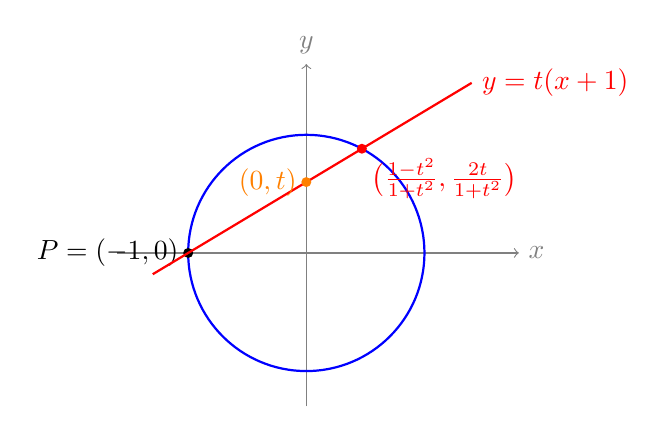
\begin{tikzpicture}[scale=1.5]
  \draw[->,gray] (-1.6,0)--(1.8,0) node[right] {$x$};
  \draw[->,gray] (0,-1.3)--(0,1.6) node[above] {$y$};
  \draw[thick,blue] (0,0) circle (1);
  \fill (-1,0) circle (1.2pt) node[left] {$P=(-1,0)$};
  \draw[thick,red] (-1.3,-0.18)--(1.4,1.44) node[right] {$y=t(x+1)$};
  % t = 0.6 : x = (1-0.36)/1.36 = 0.4706, y = 1.2/1.36 = 0.8824
  \fill[red] (0.4706,0.8824) circle (1.2pt) node[below right] {$\bigl(\frac{1-t^2}{1+t^2},\frac{2t}{1+t^2}\bigr)$};
  \fill[orange] (0,0.6) circle (1.2pt) node[left] {$(0,t)$};
\end{tikzpicture}
\caption{円の立体射影．$P$ を通る傾き $t$ の直線と円の2番目の交点が，パラメータ $t$ に対応する．$y$ 軸との交点 $(0,t)$ を見れば，円から直線への写像になっている．}
\label{fig:ch10-stereo}
\end{figure}

\begin{note}
立体射影は $\Q$ 上でも定義されるので，$t\in\Q$ に対し有理点 $(x,y)\in C(\Q)$ が得られ，逆もいえる．
$t=n/m$ を代入して分母を払えば $(m^2-n^2)^2+(2mn)^2=(m^2+n^2)^2$，すなわちピタゴラス数の一般形が得られる．
\end{note}

\begin{physbox}[立体射影と物理]
立体射影 $S^2\to\C\cup\{\infty\}=\PP^1_\C$ は物理の至るところに現れる：スピン $1/2$ の状態の Bloch 球表示，2次元共形場理論の Riemann 球，$O(3)$ 非線形シグマ模型の $\PP^1$ 模型としての記述などである．
上の計算は，円（実の円錐曲線）が「有理関数でパラメータ付けできる」ことを示している．
これは，例えば相対論的速度合成で $\tanh$ の加法定理が $t=\tanh(\eta/2)$ による有理パラメータ表示で書けることとも関係している．
\end{physbox}

\subsection{双有理変換}

多様体 $X$ から自分自身への双有理写像を\textbf{双有理変換}といい，その全体は群 $\mathrm{Bir}(X)$ をなす．
同型写像の群 $\Aut(X)$ はその部分群である．

\begin{myex}{Cremona 群}{ch10-cremonagroup}
$\mathrm{Bir}(\PP^2)$ を（平面）\textbf{Cremona 群}という．
$\Aut(\PP^2)=\PGL_3(k)$ は8次元の代数群だが，$\mathrm{Bir}(\PP^2)$ ははるかに巨大で，例えば
\[
  (x,y)\mapsto(x,\ y+p(x))\qquad(p\in k[x]\ \text{任意})
\]
（アフィン座標で表示）のような「次数無限大まで」の変換を含む．
Noether--Castelnuovo の定理によれば，$\mathrm{Bir}(\PP^2)$（$k$ 代数閉）は $\PGL_3(k)$ と標準 Cremona 変換 $\sigma$ で生成される．
\end{myex}

標準 Cremona 変換 $\sigma$ は，3点 $P_1,P_2,P_3$ を blow-up して3本の直線を blow-down する操作として理解できる（下の 10.3.4小節と図\ref{fig:ch10-cremona}）．
一般に，曲面の双有理変換はすべて blow-up と blow-down の合成で書ける（曲面の弱分解定理）．

\subsection{例：アフィン空間間の変換}

\begin{myex}{$\A^2$ の双有理自己写像}{ch10-A2bir}
$\beta:\A^2\to\A^2$，$(u,v)\mapsto(x,y)=(u,uv)$ を考える．逆は $(x,y)\mapsto(x,y/x)$ で，$x\neq0$ で定義される．
したがって $\beta$ は双有理射であり，$\{u\neq0\}\cong\{x\neq0\}$ の同型を与える．
しかし $\beta$ は直線 $\{u=0\}$ 全体を原点 $(0,0)$ に潰しており，同型ではない．
\end{myex}

この写像は，次に定義する blow-up の1つのチャートに他ならない．

\begin{mydef}{$\A^2$ の原点での blow-up}{ch10-blowup}
\[
  \widetilde{\A^2}=\mathrm{Bl}_0\A^2=\{\,((x,y),[u:v])\in\A^2\times\PP^1 \;:\; xv=yu\,\}
\]
とし，第1成分への射影を $\pi:\widetilde{\A^2}\to\A^2$ とする．これを $\A^2$ の原点での\textbf{blow-up}（爆発，ブローアップ）といい，
\[
  E=\pi^{-1}(0)=\{0\}\times\PP^1\cong\PP^1
\]
を\textbf{例外因子}（exceptional divisor）という．
\end{mydef}

条件 $xv=yu$ は「点 $(x,y)$ が方向 $[u:v]$ の直線上にある」ことを意味する．
\begin{itemize}
  \item $(x,y)\neq0$ なら方向 $[u:v]=[x:y]$ が一意に決まるので，$\pi$ は $\widetilde{\A^2}\setminus E\to\A^2\setminus\{0\}$ の同型である．とくに $\pi$ は双有理射．
  \item 原点の上では方向 $[u:v]$ は任意であり，原点は「原点を通る直線の方向全体」$\PP^1$ に置き換わる．
\end{itemize}
$\widetilde{\A^2}$ は2つのアフィンチャートで覆われる：
\[
  \{u\neq0\}:\ (x,v')\ \ (v'=v/u,\ y=xv'),\qquad \{v\neq0\}:\ (u',y)\ \ (u'=u/v,\ x=u'y).
\]
各チャートは $\A^2$ と同型で，$\pi$ は例\ref{ex:ch10-A2bir}の写像 $(x,v')\mapsto(x,xv')$ である．$E$ はチャート1で $\{x=0\}$ と表される．
とくに $\widetilde{\A^2}$ は滑らかな曲面である．

\paragraph{不確定点の解消．}
例\ref{ex:ch10-projection}の $\pi:\PP^2\dashrightarrow\PP^1$（$O$ からの射影）は，$\widetilde{\A^2}\to\PP^1$，$((x,y),[u:v])\mapsto[u:v]$ という\emph{射}になる．
すなわち blow-up は，$O$ に近づく「方向」の情報を新しい点として付け加えることで，不確定点を解消する．

\paragraph{固有変換と特異点の解消．}
曲線 $C\subset\A^2$ の $\pi^{-1}(C\setminus\{0\})$ の閉包を $C$ の\textbf{固有変換}（strict transform）$\widetilde C$ という．

\begin{myex}{結節点の解消}{ch10-nodebl}
$C:\ y^2=x^2(x+1)$（原点で結節点）．チャート1で $y=xv'$ を代入すると
\[
  x^2v'^2=x^2(x+1)\iff x^2\bigl(v'^2-x-1\bigr)=0.
\]
$x^2=0$ は例外因子 $E$（2重）であり，固有変換は $\widetilde C:\ v'^2=x+1$．これは滑らかで，$E=\{x=0\}$ と2点 $v'=\pm1$ で横断的に交わる．
原点の2本の枝（接線 $y=\pm x$）が，$E$ 上の異なる2点に引き離されたのである．
\end{myex}

\begin{myex}{尖点の解消と正規化}{ch10-cuspbl}
$C:\ y^2=x^3$（原点で尖点）．チャート1で $y=xv'$ とすると $x^2(v'^2-x)=0$，固有変換は $\widetilde C:\ x=v'^2$ で滑らか（放物線）．
$\widetilde C\cong\A^1$（座標 $v'$）であり，合成 $\widetilde C\to C$ は
\[
  v'\mapsto(x,y)=(v'^2,v'^3)
\]
となる．これは例\ref{ex:ch10-cuspbij}の $\nu$ そのものであり，$v'=y/x$ が逆の有理写像である．
こうして $\nu:\A^1\to C$ は全単射な双有理射だが同型でない射であり，$C$ の\textbf{正規化}と呼ばれる．
代数的には $k[C]=k[t^2,t^3]\subset k[t]$ で，$k[t]$ は $k[C]$ の商体 $k(t)$ における $k[C]$ の整閉包である．
\end{myex}

\begin{figure}[htbp]
\centering
\begin{tikzpicture}[scale=0.9]
  % left: node
  \begin{scope}
    \draw[->,gray] (-1.8,0)--(1.8,0);
    \draw[->,gray] (0,-1.8)--(0,1.8);
    \draw[thick,blue,domain=-1:0.6,samples=60] plot ({\x},{\x*sqrt(\x+1)});
    \draw[thick,blue,domain=-1:0.6,samples=60] plot ({\x},{-\x*sqrt(\x+1)});
    \fill (0,0) circle (2pt);
    \node at (0,-2.2) {$\A^2$：結節点を持つ $C$};
  \end{scope}
  \draw[<-,thick] (2.4,0)--(3.6,0) node[midway,above] {$\pi$};
  % right: blow-up
  \begin{scope}[xshift=6.2cm]
    \draw[very thick,red] (0,-1.8)--(0,1.8) node[above] {$E\cong\PP^1$};
    \draw[thick,blue,domain=-1.4:1.4,samples=60] plot ({\x*\x-1},{\x});
    \fill (0,1) circle (2pt) node[right] {$v'=1$};
    \fill (0,-1) circle (2pt) node[right] {$v'=-1$};
    \node at (0.4,-2.2) {$\widetilde{\A^2}$：固有変換 $\widetilde C$ は滑らか};
  \end{scope}
\end{tikzpicture}
\caption{結節点 $y^2=x^2(x+1)$ の blow-up（チャート $y=xv'$，横軸 $x$，縦軸 $v'$）．原点が例外因子 $E$ に置き換わり，2本の枝は $E$ 上の異なる2点 $v'=\pm1$ を通る滑らかな曲線 $v'^2=x+1$ に分離される．}
\label{fig:ch10-blowup}
\end{figure}

\paragraph{例外因子の自己交差数．}
$\PP^2$ の点を blow-up した曲面 $\widetilde{\PP^2}$ では，例外因子 $E$ の自己交差数は $E\cdot E=-1$ である（第9章の交差数を曲面に拡張したもの）．
実際，原点を通る直線 $L$ の固有変換 $\widetilde L$ と全変換 $\pi^*L=\widetilde L+E$ について $\pi^*L\cdot E=0$（$L$ を原点を通らない直線に動かせるため）かつ $\widetilde L\cdot E=1$ から $E\cdot E=-1$ が従う．

\subsection{双有理幾何の基本的な考え方}

双有理同値は同型より粗い分類であり，「低次元の閉集合での違いを無視する」．
その目標は次の2段階で述べられる．
\begin{enumerate}
  \item \textbf{双有理不変量}を見つけ，双有理同値類を区別する．最も基本的な不変量は関数体 $k(X)$（10.4節）であり，そのほかに滑らかな射影曲線の種数 $g$，多重種数 $P_m=\dim H^0(X,\omega_X^{\otimes m})$，小平次元などがある．
  \item 各双有理同値類の中で「最も良い」代表元（\textbf{極小モデル}）を選ぶ．曲面では $E\cdot E=-1$ となる有理曲線 $E$ を blow-down（$(-1)$ 曲線の収縮）し続けることで極小モデルに到達する．高次元ではこれが森の極小モデル理論（MMP）である．
\end{enumerate}

\begin{myex}{特異点解消}{ch10-resolution}
広中の定理（標数0）によれば，任意の多様体 $X$ に対して，滑らかな多様体 $\widetilde X$ と双有理な射影的射 $\widetilde X\to X$ が存在する（特異点解消）．
曲線の場合は正規化（例\ref{ex:ch10-cuspbl}）で十分であり，曲面以上では blow-up の繰り返しが必要になる．
特異点解消の概念は第7章で紹介した．
\end{myex}

\begin{physbox}[双有理幾何とトポロジー変化]
Calabi--Yau 3次元多様体では，ある有理曲線 $\PP^1$ を潰して特異点（conifold）を作り，別の方法でそれを解消すると，双有理同値だが同型でない Calabi--Yau 多様体が得られる（\textbf{flop}）．
Batyrev の定理によれば，双有理同値な Calabi--Yau 多様体は同じ Betti 数を持つ（さらに Hodge 数も一致することが知られている）が，三重交差数（第9章）などは一般に異なる．
弦理論では，Kähler モジュライ空間の中でこの2つの多様体の領域が滑らかにつながっており，時空のトポロジーが物理的に滑らかに変化しうること（Aspinwall--Greene--Morrison, Witten）が示された．
双有理幾何は「同じ物理を記述する異なる幾何」を理解する言葉でもある（第15章・第17章）．
\end{physbox}

\exprob{prob:ch10-5}
曲線 $C:\ y^2=x^5$ の原点での blow-up をチャート $y=xv'$ で計算し，固有変換が依然として特異であることを確かめよ．
もう一度 blow-up するとどうなるか．何回で滑らかになるか．

\exprob{prob:ch10-6}
標準 Cremona 変換 $\sigma$ について，$\sigma$ が $P_1,P_2,P_3$ を通らない一般の直線を何次の曲線に写すか答えよ．また，像曲線は $P_1,P_2,P_3$ を通ることを確かめよ．

% ------------------------------------------------------------
\section{関数体}
% ------------------------------------------------------------

\subsection{多様体上の有理関数}

10.2.3小節で定義した有理関数をもう少し具体的に記述する．

\begin{myprop}{有理関数の具体的記述}{ch10-ratdesc}
\begin{enumerate}
  \item $X$ がアフィン多様体のとき，$X$ 上の有理関数は $g/h$（$g,h\in k[X]$, $h\neq0$）の形に書け，$g/h=g'/h'\iff gh'=g'h$ in $k[X]$．
  \item $X\subset\PP^n$ が射影多様体のとき，$X$ 上の有理関数は $G/H$（$G,H$ は同じ次数の同次多項式で $H\notin\Ideal(X)$）の形に書け，$G/H=G'/H'\iff GH'-G'H\in\Ideal(X)$．
\end{enumerate}
\end{myprop}

\begin{proof}[証明の概略]
(1) $f\in\OO_X(U)$ について，$U$ に含まれる基本開集合 $D(h)$ を取ると，$\OO_X(D(h))=k[X]_h$（第6章の局所化）なので $f=g/h^m$．
(2) は (1) を $X\cap U_i$ に適用し，$x_i$ のべきで同次化すればよい．
\end{proof}

\begin{myex}{有理関数と定義域}{ch10-ratdom}
$X=\Zero(xz-y^2)\subset\PP^2$ 上の有理関数 $f=x/y$ を考える．$X$ 上では $xz=y^2$ なので $x/y=y/z$ でもある．
$x/y$ は $y\neq0$ で，$y/z$ は $z\neq0$ で正則であり，あわせて $f$ は $X\setminus\{[1:0:0]\}$ で正則．
$[1:0:0]$ では $x/y=y/z$ の分母がいずれも0になり，実際そこは $f$ の極である（$1/f=y/x$ は $[1:0:0]$ の近傍で正則で0になる）．
\end{myex}

\subsection{関数体の定義}

\begin{mydef}{関数体}{ch10-funcfield}
多様体 $X$ 上の有理関数全体のなす体を $X$ の\textbf{関数体}といい，$k(X)$ と書く．
\end{mydef}

命題\ref{prop:ch10-ratdesc}から次がわかる．

\begin{myprop}{関数体の計算}{ch10-ffcomp}
\begin{enumerate}
  \item $X$ がアフィンなら $k(X)=\Frac k[X]$（座標環の商体）．
  \item $U\subset X$ が空でない開集合なら $k(U)=k(X)$．とくに射影多様体 $X$ について $k(X)=k(X\cap U_i)$．
  \item $X\subset\PP^n$ が射影多様体なら，$k(X)$ は同次座標環 $S(X)$ の商体の次数0部分 $\{G/H:\deg G=\deg H\}$ に等しい．
  \item $k(X)$ の $k$ 上の超越次数は $\dim X$ に等しい．
\end{enumerate}
\end{myprop}

(4) は第7章の「次元 = 座標環の商体の超越次数」をアフィン開集合に適用したものである．

\begin{myex}{関数体の例}{ch10-ffex}
\begin{enumerate}
  \item $k(\A^n)=k(\PP^n)=k(x_1,\dots,x_n)$（$n$ 変数有理関数体）．
  \item 円 $C:\ x^2+y^2=1$ では $k(C)=\Frac\bigl(k[x,y]/(x^2+y^2-1)\bigr)$．立体射影の $t=y/(x+1)$ を使うと $x,y$ は $t$ の有理式で書けるので $k(C)=k(t)$．
  \item 尖点曲線 $C:\ y^2=x^3$ では $t=y/x\in k(C)$ が $x=t^2$, $y=t^3$ を満たすので $k(C)=k(t)$．$k[C]=k[t^2,t^3]\subsetneq k[t]$ と比べると，座標環は違っても関数体は同じである．
  \item 楕円曲線 $E:\ y^2=x^3+ax+b$ では $k(E)=k(x)[y]/(y^2-x^3-ax-b)$ であり，$k(x)$ の2次拡大．$k(E)$ は純超越拡大 $k(t)$ と同型ではない（10.4.4小節）．
\end{enumerate}
\end{myex}

\subsection{関数体と多様体}

双有理幾何の基本定理は，「双有理同値類は関数体で完全に決まる」というものである．

\begin{mythm}{双有理同値と関数体}{ch10-birff}
多様体 $X,Y$ について次は同値である．
\begin{enumerate}
  \item $X$ と $Y$ は双有理同値である．
  \item $k$ 上の体の同型 $k(X)\cong k(Y)$ が存在する．
  \item 空でない開集合 $U\subset X$, $V\subset Y$ で $U\cong V$ となるものが存在する．
\end{enumerate}
より精密に，支配的有理写像 $\varphi:X\dashrightarrow Y$ と $k$ 上の体の準同型 $k(Y)\to k(X)$ は，$\varphi\mapsto\varphi^*$ によって1対1に対応する．
\end{mythm}

\begin{proof}[証明の概略]
\textbf{有理写像から準同型へ}．$\varphi$ が支配的なら，$f\in k(Y)$ の定義域 $V$ に対し $\varphi^{-1}(V)$ は空でない開集合で，$\varphi^*f=f\circ\varphi$ はそこで正則．よって $\varphi^*:k(Y)\to k(X)$ が定まる．体の準同型なので自動的に単射．

\textbf{準同型から有理写像へ}．$\theta:k(Y)\to k(X)$ を $k$ 上の準同型とする．$Y$ をアフィン開集合に取り替えて（$k(Y)$ は変わらない）$Y\subset\A^m$，$k[Y]=k[y_1,\dots,y_m]/\Ideal(Y)$ とする．
$\theta(y_i)\in k(X)$ は有限個の有理関数なので，それらがすべて正則になるアフィン開集合 $U\subset X$ が取れる．
すると $\theta$ は $k$ 代数の準同型 $k[Y]\to\OO_X(U)=k[U]$ を与え，第5章の対応により射 $U\to Y$，すなわち有理写像 $X\dashrightarrow Y$ を与える．$\theta$ が単射なのでこの射は支配的である．

\textbf{同値性}．(1)$\Leftrightarrow$(3) は命題\ref{prop:ch10-biropen}．(1)$\Rightarrow$(2)：$\varphi^*$ と $\psi^*$ が互いに逆．(2)$\Rightarrow$(1)：同型とその逆から上の構成で互いに逆の有理写像が得られる．
\end{proof}

この定理により，次の対応（圏の反変同値）が得られる：
\[
  \left\{\begin{array}{c}\text{多様体と}\\\text{支配的有理写像}\end{array}\right\}
  \;\longleftrightarrow\;
  \left\{\begin{array}{c}k\text{ 上の有限生成体拡大 } K\\\text{と $k$ 上の体の準同型}\end{array}\right\}^{\mathrm{op}}.
\]
これはアフィン多様体と座標環の対応（第5章）の双有理版である．
任意の有限生成体拡大 $K/k$ は $K=k(a_1,\dots,a_m)$ と書け，$k[a_1,\dots,a_m]$ を座標環とするアフィン多様体の関数体として実現される．

\begin{myex}{関数体の包含と写像}{ch10-ffmap}
$\varphi:\A^1\to\A^1$，$t\mapsto t^2$ に対応する準同型は $k(s)\to k(t)$，$s\mapsto t^2$ で，$k(t)$ は $k(t^2)$ の2次拡大．
拡大次数 $[k(X):\varphi^*k(Y)]=2$ は，$\varphi$ の一般のファイバーの点の数 2 に等しい（$\mathrm{char}\,k\neq2$）．
一般に，同じ次元の多様体の間の支配的射 $\varphi$ に対し $[k(X):k(Y)]$ を $\varphi$ の\textbf{次数}といい，双有理 $\iff$ 次数1 である．
\end{myex}

\subsection{関数体による幾何学的分類}

関数体の観点から，多様体を「どれほど有理的か」で分類できる．

\begin{mydef}{有理性}{ch10-rationality}
$n$ 次元多様体 $X$ が\textbf{有理的}であるとは $k(X)\cong k(t_1,\dots,t_n)$（純超越拡大）となることをいう．
また支配的有理写像 $\PP^n\dashrightarrow X$ が存在するとき（$k(X)\subset k(t_1,\dots,t_n)$ と埋め込めるとき）\textbf{単有理的}という．
\end{mydef}

\paragraph{曲線の場合．}
1次元の場合，状況は非常にきれいである．
\begin{mythm}{曲線と関数体}{ch10-curves}
$k$ 上の超越次数1の有限生成体 $K$ に対し，$k(C)\cong K$ となる滑らかな射影曲線 $C$ が同型を除いて一意に存在する．
とくに滑らかな射影曲線の間では，双有理同値と同型は同じである．
\end{mythm}

後半は命題\ref{prop:ch10-curveext}から従う：双有理写像 $C\dashrightarrow C'$ とその逆はともに射に延び，合成は稠密開集合上で恒等なので恒等射である．
したがって曲線の双有理分類は，滑らかな射影曲線の同型分類に一致する．

\begin{myex}{有理曲線と楕円曲線}{ch10-ellnotrational}
\begin{itemize}
  \item 円錐曲線・尖点3次曲線・結節点3次曲線の関数体はすべて $k(t)$ であり，有理曲線である．これらの正規化はすべて $\PP^1$ である．
  \item 滑らかな3次曲線 $E$ は有理的でない．実際，$E$ は種数1（$\C$ 上ではトーラス）であり，種数は双有理不変量だからである．
  代数的には，$k(t)$ の部分体はすべて再び純超越的（Lüroth の定理）なので，$E$ は単有理的ですらない．
\end{itemize}
\end{myex}

\paragraph{高次元の場合．}
曲面になると，双有理同値類の中に無限個の非同型な滑らかな射影曲面（点の blow-up を繰り返したもの）が含まれる．
それでも，Castelnuovo の判定法（$q=P_2=0$ なら有理的）のように，双有理不変量による美しい分類が存在する．
3次元以上では，単有理的だが有理的でない多様体（例えば滑らかな3次3次元超曲面；Clemens--Griffiths）が存在し，有理性の問題は現在でも活発な研究対象である．

\begin{physbox}[関数体と「場の代数」]
関数体 $k(X)$ は，$X$ 上の「ほとんど至るところで定義された観測量」の代数とみなせる．
$X$ が $\PP^1$ と双有理であることは，全観測量が1つの「場」$t$ の有理関数として書けることを意味し，物理系の\emph{有理的パラメータ化}（例：古典解の有理的な表示，可積分系の有理的な保存量）と結びつく．
逆に楕円曲線のように有理的でない場合，パラメータ化には楕円関数のような超越関数が必要になる．
これは単振り子の厳密解が楕円関数で書かれる事情の幾何学的な背景である．
\end{physbox}

\exprob{prob:ch10-7}
$X=\Zero(xy-zw)\subset\PP^3$ の関数体が $k(s,t)$（2変数の純超越拡大）と同型であることを示し，$X$ と $\PP^2$ の間の双有理写像を具体的に与えよ．

% ------------------------------------------------------------
\section{圏論的な視点}
% ------------------------------------------------------------

ここまでに現れた「多様体と射」「座標環と準同型」「関数体と体準同型」の対応は，すべて圏と関手の言葉で統一的に表現できる．
圏論の基礎は付録Gにまとめてあるので，ここでは必要最小限の言葉を導入し，代数幾何での意味に焦点を当てる．

\subsection{対象と射}

\begin{mydef}{圏}{ch10-category}
\textbf{圏} $\mathcal C$ とは，次のデータからなるものである．
\begin{enumerate}
  \item 対象の集まり $\mathrm{Ob}(\mathcal C)$．
  \item 対象の組 $X,Y$ ごとの射の集合 $\Hom_{\mathcal C}(X,Y)$．
  \item 合成 $\Hom(Y,Z)\times\Hom(X,Y)\to\Hom(X,Z)$，$(g,f)\mapsto g\circ f$ で，結合法則 $h\circ(g\circ f)=(h\circ g)\circ f$ を満たすもの．
  \item 各対象 $X$ の恒等射 $\mathrm{id}_X$ で，$f\circ\mathrm{id}_X=f=\mathrm{id}_Y\circ f$ を満たすもの．
\end{enumerate}
\end{mydef}

\begin{myex}{本講義に現れる圏}{ch10-catex}
\begin{center}
\renewcommand{\arraystretch}{1.3}
\begin{tabular}{lll}
\hline
圏 & 対象 & 射 \\
\hline
$\mathbf{Set}$ & 集合 & 写像 \\
$\mathbf{Top}$ & 位相空間 & 連続写像 \\
$\mathbf{Var}_k$ & 準射影多様体 & 射（10.1節） \\
$\mathbf{AffAlg}_k$ & アフィン代数的集合 & 射（多項式写像） \\
$\mathbf{Alg}_k^{\mathrm{red}}$ & 有限生成被約 $k$ 代数 & $k$ 代数の準同型 \\
$\mathbf{Var}_k^{\mathrm{dom}}$ & 多様体 & 支配的有理写像 \\
$\mathbf{Field}_k$ & $k$ 上有限生成な体 & $k$ 上の体準同型 \\
\hline
\end{tabular}
\end{center}
\end{myex}

圏の中での\textbf{同型}は「逆射を持つ射」として定義される．定義\ref{def:ch10-iso}はまさに $\mathbf{Var}_k$ における同型であり，双有理写像は $\mathbf{Var}_k^{\mathrm{dom}}$ における同型である．
このように，「どの圏で考えるか」によって「同じ」の意味が変わる．

\subsection{代数的集合の圏}

アフィン代数的集合（既約とは限らない）の圏 $\mathbf{AffAlg}_k$ を考える．対象は $X\subset\A^n$（ある $n$ について），射は多項式写像 $X\to Y$ である．
各 $X$ に座標環 $k[X]=k[x_1,\dots,x_n]/\Ideal(X)$ を対応させると，零点定理により $\Ideal(X)$ は根基イデアルなので，$k[X]$ は\textbf{有限生成被約 $k$ 代数}である（被約 = 零でないべき零元を持たない）．

\begin{mydef}{関手}{ch10-functor}
圏 $\mathcal C$ から $\mathcal D$ への\textbf{（共変）関手} $\mathcal F$ とは，対象 $X$ に対象 $\mathcal F(X)$ を，射 $f:X\to Y$ に射 $\mathcal F(f):\mathcal F(X)\to\mathcal F(Y)$ を対応させ，
\[
  \mathcal F(g\circ f)=\mathcal F(g)\circ\mathcal F(f),\qquad \mathcal F(\mathrm{id}_X)=\mathrm{id}_{\mathcal F(X)}
\]
を満たすものである．射の向きを反転させ $\mathcal F(f):\mathcal F(Y)\to\mathcal F(X)$, $\mathcal F(g\circ f)=\mathcal F(f)\circ\mathcal F(g)$ となるものを\textbf{反変関手}という．
\end{mydef}

\begin{myex}{座標環関手}{ch10-coordfunctor}
$X\mapsto k[X]$，$(\varphi:X\to Y)\mapsto(\varphi^*:k[Y]\to k[X])$ は反変関手
\[
  k[-]:\mathbf{AffAlg}_k\to\mathbf{Alg}_k^{\mathrm{red}}
\]
である．実際 $(\psi\circ\varphi)^*=\varphi^*\circ\psi^*$，$\mathrm{id}^*=\mathrm{id}$（命題\ref{prop:ch10-composition}の直後の注意）．
\end{myex}

\subsection{反変性}

第5章の結果を圏論の言葉で言い換えると，次のようになる．

\begin{mythm}{アフィン代数的集合と被約代数の反変同値}{ch10-antiequiv}
$k$ を代数閉体とする．座標環関手 $k[-]$ は圏の反変同値
\[
  \mathbf{AffAlg}_k\;\simeq\;\bigl(\mathbf{Alg}_k^{\mathrm{red}}\bigr)^{\mathrm{op}}
\]
を与える．すなわち
\begin{enumerate}
  \item（充満忠実）任意の $X,Y$ について $\Hom(X,Y)\to\Hom_{k\text{-alg}}(k[Y],k[X])$，$\varphi\mapsto\varphi^*$ は全単射である．
  \item（本質的全射）任意の有限生成被約 $k$ 代数 $A$ に対し，$k[X]\cong A$ となるアフィン代数的集合 $X$ が存在する．
\end{enumerate}
この同値のもとで，アフィン\emph{多様体}（既約）は有限生成な $k$ 上の整域に対応する．
\end{mythm}

\begin{proof}[証明の概略]
(1)は第5章で示した：$\theta:k[Y]\to k[X]$ に対し $\varphi=(\theta(y_1),\dots,\theta(y_m)):X\to Y$ と置けば $\varphi^*=\theta$．
(2)：$A=k[x_1,\dots,x_n]/I$ と表すと，$A$ が被約なので $I=\sqrt I$．零点定理より $\Ideal(\Zero(I))=\sqrt I=I$ なので，$X=\Zero(I)$ とすれば $k[X]=A$．
\end{proof}

逆向きの関手は，代数 $A$ から点の集合
\[
  X_A=\Hom_{k\text{-alg}}(A,k)\;\cong\;\{A\text{ の極大イデアル}\}
\]
を作る操作である（弱零点定理により $k$ 値の点と極大イデアルが対応する）．
点 $p\in X$ は「評価写像」$\mathrm{ev}_p:k[X]\to k$，$f\mapsto f(p)$ と同一視される．
これは，状態が観測量の代数上の線形汎関数として与えられるという量子論の考え方（Gelfand--Naimark の定理の代数幾何版）と同じ構造である．

\begin{figure}[htbp]
\centering
\begin{tikzcd}[column sep=large,row sep=large]
X \arrow[r,"\varphi"] \arrow[d,mapsto] & Y \arrow[r,"\psi"] \arrow[d,mapsto] & Z \arrow[d,mapsto]\\
k[X] & k[Y] \arrow[l,"\varphi^*"'] & k[Z] \arrow[l,"\psi^*"']
\end{tikzcd}
\caption{座標環関手の反変性．幾何側の射の向きが代数側では反転する．}
\label{fig:ch10-contra}
\end{figure}

\subsection{幾何学と代数の対応の圏論的理解}

反変同値のもとで，幾何学的な概念は代数的な概念に翻訳される．これまでの章の結果を辞書としてまとめる．

\begin{center}
\renewcommand{\arraystretch}{1.35}
\begin{tabular}{ll}
\hline
幾何（アフィン代数的集合） & 代数（有限生成被約 $k$ 代数） \\
\hline
点 $p\in X$ & 極大イデアル $\m_p\subset k[X]$，準同型 $k[X]\to k$ \\
閉部分集合 $Z\subset X$ & 根基イデアル $\Ideal(Z)$，全射 $k[X]\to k[Z]$ \\
既約 & 整域 \\
基本開集合 $D(f)$ & 局所化 $k[X]_f$ \\
点の局所的な様子 & 局所環 $\OO_{X,p}=k[X]_{\m_p}$ \\
直積 $X\times Y$ & テンソル積 $k[X]\otimes_kk[Y]$ \\
支配的な射 & 単射な準同型 \\
閉埋め込み & 全射な準同型 \\
1点 & $k$ \\
空集合 & 零環 $0$ \\
\hline
\end{tabular}
\end{center}

例えば「直積 $\leftrightarrow$ テンソル積」は，圏論的には「直積（積の普遍性）が反変同値で余積（テンソル積の普遍性）に移る」という一般的な事実の現れである．
$X\times Y$ が積であるとは，任意の $Z$ と射 $Z\to X$, $Z\to Y$ に対し $Z\to X\times Y$ がただ1つ存在すること（普遍性）であり，代数側では $k[X]\to C$, $k[Y]\to C$ から $k[X]\otimes k[Y]\to C$ がただ1つ定まることに対応する．

\begin{myex}{$\A^1\times\A^1=\A^2$}{ch10-product}
$k[x]\otimes_kk[y]\cong k[x,y]$ なので $\A^1\times\A^1\cong\A^2$．
ただし Zariski 位相は積位相ではない（$\A^2$ の閉集合 $\Zero(y-x^2)$ は積位相では閉集合でない）．
「積」は位相空間としてではなく，圏（$\mathbf{AffAlg}_k$）の中で普遍性によって定義すべきものである．これは圏論的視点の利点の一例である．
\end{myex}

\subsection{圏論的言語の利点}

圏論的な言葉を使うと何が得られるのか．代数幾何の発展にとって決定的だった点を3つ挙げる．

\paragraph{(1) 対象を「射」で理解する．}
対象 $X$ はそれへの射の全体 $\Hom(-,X)$ で決まる（米田の補題；付録G）．
例えば $X$ の点は $\Hom(\{pt\},X)=\Hom_{k\text{-alg}}(k[X],k)$ である．
$k$ を他の環 $R$ に取り替えて $X(R)=\Hom(k[X],R)$ を考えることで「$R$ 値の点」という概念が得られ，$R=k[\varepsilon]/(\varepsilon^2)$ と取れば接ベクトル（第7章）が，$R$ を一般の環にすればスキームの関手的な見方が得られる．
これが第12章のスキーム論の出発点である．

\paragraph{(2) 構成を普遍性で特徴付ける．}
積・ファイバー積・商・blow-up などは，具体的な方程式ではなく普遍性によって特徴付けられる．
これにより「座標の取り方によらない」ことが自動的に保証され，貼り合わせ（第11章の層）による大域的な構成が可能になる．

\paragraph{(3) 異なる分野の間の「同値」を述べる．}
「幾何と代数は同じものの2つの見方である」という主張は，「2つの圏が（反変）同値である」と正確に定式化できる．
本節の定理\ref{thm:ch10-antiequiv}と定理\ref{thm:ch10-birff}はその典型である．

\begin{physbox}[双対性と圏の同値]
現代の数理物理では，「双対性」はしばしば圏の同値として定式化される．
\begin{itemize}
  \item ホモロジー的ミラー対称性（Kontsevich）：Calabi--Yau 多様体 $X$ 上の連接層の導来圏 $D^b(\mathrm{Coh}\,X)$（B ブレーンの圏）と，ミラー $\check X$ の深谷圏（A ブレーンの圏）が同値になる，という予想．
  \item D ブレーンは圏の対象，ブレーン間の開弦の状態は射の空間 $\Hom$ であり，弦の相互作用は射の合成に対応する．
\end{itemize}
本節で見た「アフィン多様体 $\leftrightarrow$ 可換代数」という単純な反変同値は，このような壮大な対応の最も初等的なモデルである．
物理的には「空間（幾何）」と「観測量の代数」のどちらを基本とみなしても同じ情報を持つ，という主張であり，非可換幾何の発想の出発点でもある．
\end{physbox}

\exprob{prob:ch10-8}
定理\ref{thm:ch10-antiequiv}の反変同値のもとで，$\A^1$ から自分自身への射のなす集合 $\Hom(\A^1,\A^1)$ が $k[t]$ と1対1に対応することを確認せよ．
また，2点からなる代数的集合 $\{0,1\}\subset\A^1$ の座標環が $k\times k$ と同型であることを示し，これが「互いに交わらない2つの1点の和」が代数側で「直積」になることの例であることを説明せよ．

\section*{問題の解答}
\addcontentsline{toc}{section}{問題の解答}

\exsol{prob:ch10-1}
$\PP^3$ の同次座標を $[a:b:c:d]$ とする．$s^3,t^3$ は同時に消えないので，命題\ref{prop:ch10-localform}により $\varphi$ は射である．
命題\ref{prop:ch10-morprop}(3) より像 $T=\varphi(\PP^1)$ は $\PP^3$ の閉集合であり，既約集合の像なので既約，すなわち射影多様体である．$\varphi$ は $T$ への射 $\PP^1\to T$ とみなせる．
$T$ の点 $[s^3:s^2t:st^2:t^3]$ の座標は
\[
  ad-bc=s^3t^3-s^2t\cdot st^2=0
\]
を満たす（実は $T=\Zero(ac-b^2,\ bd-c^2,\ ad-bc)$ であるが，以下では使わない）．

\textbf{逆写像の局所表示．}$T$ を2つの開集合
\[
  V_1=T\cap\{(a,b)\neq(0,0)\},\qquad V_2=T\cap\{(c,d)\neq(0,0)\}
\]
で覆う．実際 $T$ の点で $a=b=0$ なら $s^3=0$ より $s=0$，したがって $t\neq0$ で $d=t^3\neq0$ である．
\[
  \psi(p)=\begin{cases}[a:b] & (p\in V_1)\\ [c:d] & (p\in V_2)\end{cases}
\]
と定める．$p\in V_1\cap V_2$ では，$(a,b)$ と $(c,d)$ はともに零でなく，$ad-bc=0$ より $(a,b)$ と $(c,d)$ は比例するので $[a:b]=[c:d]$ であり，$\psi$ は well-defined である．
各 $V_i$ 上で $\psi$ は同じ次数（1次）の同次多項式の組で，$V_i$ 上で同時には消えないもので表されているから，命題\ref{prop:ch10-localform}により $\psi:T\to\PP^1$ は射である（例\ref{ex:ch10-conicproj}と同じ形の構成である）．

\textbf{互いに逆であること．}$q=[s:t]\in\PP^1$ について，$s\neq0$ なら $\varphi(q)\in V_1$ で $\psi(\varphi(q))=[s^3:s^2t]=[s:t]$，$t\neq0$ なら $\varphi(q)\in V_2$ で $\psi(\varphi(q))=[st^2:t^3]=[s:t]$．よって $\psi\circ\varphi=\mathrm{id}_{\PP^1}$．
また $p\in T$ は $p=\varphi(q)$ と書けるので $\varphi(\psi(p))=\varphi(\psi(\varphi(q)))=\varphi(q)=p$，すなわち $\varphi\circ\psi=\mathrm{id}_T$．
以上より $\varphi:\PP^1\to T$ は同型である．
なお，ここで用いた2つの表示はそれぞれ1点で定義されない（$[a:b]$ は $[0:0:0:1]$ で，$[c:d]$ は $[1:0:0:0]$ で）ので，両方を併用する局所的な表示が必要になっている．

\exsol{prob:ch10-2}
\textbf{同型であること．}$\A^1\setminus\{0\}$ は $\A^1$ の開集合なので準射影多様体であり，$1/t$ はその上の正則関数である．
命題\ref{prop:ch10-morprop}(2) により
\[
  \varphi:\A^1\setminus\{0\}\to\A^2,\qquad t\mapsto(t,1/t)
\]
は射で，$t\cdot(1/t)=1$ より像は $H$ に含まれる．逆向きに
\[
  \psi:H\to\A^1\setminus\{0\},\qquad (x,y)\mapsto x
\]
を考える．これは多項式写像 $H\to\A^1$ であり，$H$ 上では $xy=1$ より $x\neq0$ なので値は開集合 $\A^1\setminus\{0\}$ に入る（開部分多様体の開集合と正則関数は $\A^1$ のものと同じなので，これは $\A^1\setminus\{0\}$ への射である）．
$\psi(\varphi(t))=t$，また $(x,y)\in H$ なら $y=1/x$ なので $\varphi(\psi(x,y))=(x,1/x)=(x,y)$．よって $\varphi$ は同型で $\A^1\setminus\{0\}\cong H$．

\textbf{大域的正則関数の環．}同型 $\varphi$ の引き戻し $\varphi^*$ は環同型 $\OO(H)\to\OO(\A^1\setminus\{0\})$ を与え（逆は $\psi^*$），$H$ はアフィン多様体なので $\OO(H)=k[H]=k[x,y]/(xy-1)$．
$k$ 代数の準同型 $k[x,y]\to k[t,t^{-1}]$，$x\mapsto t$，$y\mapsto t^{-1}$ は全射で $xy-1$ を $0$ に送る．
$k[x,y]/(xy-1)$ では $xy=1$ を使って各単項式 $x^iy^j$ を $x^{i-j}$（$i\ge j$）または $y^{j-i}$（$i<j$）に書き換えられるので，任意の元は $p(x)+q(y)$（$q(0)=0$）の形に書ける．その像 $p(t)+q(t^{-1})$ が $0$ なら，$t$ の非負べきと負べきは独立なので $p=q=0$．したがって
\[
  \OO(\A^1\setminus\{0\})\cong k[x,y]/(xy-1)\cong k[t,t^{-1}]
\]
（具体的には $\varphi^*$ で $x\mapsto t$，$y\mapsto 1/t$）．

\textbf{$\A^1$ と同型でないこと．}多様体の同型 $X\cong Y$ があれば，引き戻しにより $k$ 代数の同型 $\OO(Y)\cong\OO(X)$ が得られる．
$\OO(\A^1)=k[t]$ の単元は $k^\times$ のみである（次数を比べよ）．一方 $k[t,t^{-1}]$ では $t$ が単元で，定数ではない．
仮に $k$ 代数の同型 $\theta:k[t,t^{-1}]\to k[t]$ があれば，$\theta(t)$ は $k[t]$ の単元なので定数 $c\in k^\times$ となり，$\theta(t-c)=0$．$\theta$ は単射なので $t=c$ となり矛盾．
よって $\A^1\setminus\{0\}\not\cong\A^1$ である．幾何学的には，$t$ は「零点をもたない非定数関数」であり，そのようなものは $\A^1$ 上には存在しない．

\exsol{prob:ch10-3}
$F_0=x^2$，$F_1=xy$，$F_2=z^2$ と置く．これらが同時に消えるのは $x=z=0$，すなわち点 $p=[0:1:0]$ のみである．したがって $\PP^2\setminus\{p\}\subset\mathrm{dom}(\varphi)$ である．

\textbf{$p$ は真の不確定点である．}$p$ の開近傍 $V$ 上で $\varphi=[G_0:G_1:G_2]$（$G_i$ は同じ次数の同次多項式）と表されたとする．
$V$ と $\PP^2\setminus\{p\}$ の共通部分（空でない開集合，したがって稠密）上で $[G_0:G_1:G_2]=[F_0:F_1:F_2]$ なので，$G_iF_j-G_jF_i$ はこの稠密開集合上で消え，多項式として $0$ である．
とくに $G_0z^2=G_2x^2$．$k[x,y,z]$ は UFD で $x^2$ と $z^2$ は互いに素なので $x^2\mid G_0$，$G_0=Ax^2$ と書け，$G_2=Az^2$．さらに $G_1x^2=G_0xy=Ax^3y$ より $G_1=Axy$．
よって $(G_0,G_1,G_2)=A\cdot(x^2,xy,z^2)$ であり，$G_i$ はすべて $p$ で消える．すなわち $p$ のまわりで $\varphi$ を定義する表示は存在しない．
直観的には，アフィンチャート $y=1$ で $p$ に近づくとき，曲線 $x=cz^2$ に沿えば
\[
  \varphi=[c^2z^4:cz^2:z^2]=[c^2z^2:c:1]\ \longrightarrow\ [0:c:1]\qquad(z\to0)
\]
となり，極限が $c$ に依存する．

以上より，不確定点は $[0:1:0]$ のただ1点である．

\textbf{支配的であること．}目標の $\PP^2$ の座標を $[X:Y:Z]$ とする．$X\neq0$ の点 $[1:a:b]$ に対し，$\beta^2=b$ となる $\beta\in k$（$k$ は代数閉）を取れば
\[
  \varphi([1:a:\beta])=[1:a:\beta^2]=[1:a:b].
\]
よって $\varphi$ の像は稠密開集合 $\{X\neq0\}$ を含み，$\varphi$ は支配的である．
（なお直線 $\{x=0\}$ 上では $\varphi=[0:0:z^2]=[0:0:1]$ であり，この直線は1点に潰される．また一般の点の逆像は $[1:a:\pm\beta]$ の2点で，$\varphi$ は次数2の支配的有理写像である．）

\exsol{prob:ch10-4}
\textbf{代数的な書き換え．}$E$ 上では $y^2z=x^3+xz^2=x(x^2+z^2)$ である．したがって
\[
  x\cdot(x^2+z^2)-z\cdot y^2=0\quad(E\text{ 上})
\]
であり，命題\ref{prop:ch10-ratdesc}(2) の判定法により，$E$ 上の有理写像として
\[
  [x:z]=[y^2:x^2+z^2]
\]
が成り立つ（両辺の比 $x/z$ と $y^2/(x^2+z^2)$ が有理関数として等しい）．右辺は $O=[0:1:0]$ で $y^2=1\neq0$ なので $O$ で定義され，
\[
  \pi_O(O)=[1:0]
\]
である．

\textbf{命題\ref{prop:ch10-curveext}の手順による確認．}アフィンチャート $y=1$ で $E$ は $f(x,z)=z-x^3-xz^2=0$，$O$ は原点である．
$\partial f/\partial z=1-2xz$ は原点で $1\neq0$ なので $E$ は $O$ で滑らかで，接線は $z=0$，局所パラメータとして $x$ が取れる．
方程式を $z(1-xz)=x^3$ と書くと，$1-xz$ は $O$ で単元なので $z=x^3\cdot(1-xz)^{-1}$，すなわち $z$ の $O$ での位数は $3$，$x$ の位数は $1$ である．
よって $\pi_O=[x:z]$ の成分の位数の最小値は $1$ で，$x$ で割ると
\[
  \pi_O=[1:z/x]=[1:x^2(1-xz)^{-1}]\ \xrightarrow{\ O\ }\ [1:0].
\]
同じ答え $\pi_O(O)=[1:0]$ が得られる．

幾何学的には，$\pi_O$ は $O$ を通る直線（$x=\lambda z$ の形）でファイバーを読む写像であり，$O$ での値は $O$ における接線 $z=0$（$[x:z]=[1:0]$ に対応）である．
$z=0$ は $E$ と $O$ で3重に接する（$z$ の位数が $3$）ので，$O$ は $E$ の変曲点である．

\exsol{prob:ch10-5}
\textbf{1回目の blow-up．}チャート1で $y=xv'$ を代入すると
\[
  x^2v'^2=x^5\iff x^2\bigl(v'^2-x^3\bigr)=0
\]
となる．$x^2=0$ は例外因子 $E_1=\{x=0\}$（2重）であり，固有変換は
\[
  C_1:\ v'^2=x^3
\]
である．これは $(x,v')=(0,0)$ で尖点をもつ曲線（例\ref{ex:ch10-cuspbij}と同じ形）であり，依然として特異である．
もう一方のチャート $x=u'y$ では $y^2=u'^5y^5\iff y^2(1-u'^5y^3)=0$ で，固有変換 $u'^5y^3=1$ は $E_1=\{y=0\}$ と交わらないので，新しい点は現れない．

\textbf{2回目の blow-up．}$C_1$ の特異点 $(x,v')=(0,0)$ で blow-up する．チャート $v'=xw$ で
\[
  x^2w^2=x^3\iff x^2(w^2-x)=0
\]
となり，固有変換は
\[
  C_2:\ x=w^2
\]
で，これは滑らかな曲線（放物線，$\cong\A^1$）である．もう一方のチャート $x=u''v'$ では $v'^2=u''^3v'^3\iff v'^2(1-u''^3v')=0$ で，固有変換は例外因子 $\{v'=0\}$ と交わらない．

したがって \textbf{2回} の blow-up で滑らかになる．$C_2\cong\A^1$（座標 $w$）から $C$ への合成写像は
\[
  w\mapsto(x,v')=(w^2,w^3)\mapsto(x,y)=(x,xv')=(w^2,w^5)
\]
であり，$w=v'/x=y/x^2$ が逆の有理写像である．これは $C$ の正規化 $\A^1\to C$ にほかならない（例\ref{ex:ch10-cuspbl}と比較せよ）．
一般に $y^2=x^{2m+1}$ では，1回の blow-up ごとに $y^2=x^{2m+1}\to v'^2=x^{2m-1}$ と指数が2ずつ下がるので，$m$ 回で滑らかになる．

\exsol{prob:ch10-6}
直線 $L:\ ax+by+cz=0$ とする．$L$ が $P_1=[1:0:0]$ を通る $\iff a=0$ であり，同様に $P_2\iff b=0$，$P_3\iff c=0$ である．よって仮定より $abc\neq0$．

\textbf{像の方程式．}$\sigma$ の不確定点は $P_1,P_2,P_3$ のみ（例\ref{ex:ch10-cremona}）なので，$\sigma$ は $L$ 全体で定義され，$\sigma|_L:L\to\PP^2$ は射である．
$p=[x:y:z]\in L$ で $xyz\neq0$ のとき，像 $[X:Y:Z]=[yz:xz:xy]$ は $xyz\neq0$ を満たし，$\sigma$ は対合なので $[x:y:z]=\sigma([X:Y:Z])=[YZ:XZ:XY]$．これを $L$ の方程式に代入すると
\[
  C:\ aYZ+bXZ+cXY=0.
\]
したがって $\sigma(L\cap\{xyz\neq0\})\subset C$．$C$ は閉集合で，$L\cap\{xyz\neq0\}$ は $L$ で稠密なので，連続性により $\sigma(L)\subset C$．

\textbf{像は2次曲線 $C$ 全体．}$C$ の対称行列は（$\mathrm{char}\,k\neq2$ として）
\[
  \frac12\begin{pmatrix}0&c&b\\ c&0&a\\ b&a&0\end{pmatrix},\qquad \det=\frac{abc}{4}\neq0
\]
なので $C$ は非退化，とくに既約な2次曲線である．
一方，$\sigma(L)$ は命題\ref{prop:ch10-morprop}(1)(3) により既約な閉集合で，$\sigma$ は $\{xyz\neq0\}$ 上で単射（対合）なので無限集合，すなわち曲線である．既約曲線 $C$ に含まれる既約曲線なので $\sigma(L)=C$．
よって $\sigma$ は一般の直線を\textbf{2次曲線}（円錐曲線）に写す．
次数は次のようにも確かめられる：$L$ をパラメータ表示 $[x:y:z]=[\ell_0(u,v):\ell_1(u,v):\ell_2(u,v)]$（$\ell_i$ は1次式）すると，$\sigma|_L=[\ell_1\ell_2:\ell_0\ell_2:\ell_0\ell_1]$ は共通零点をもたない2次式の組である．

\textbf{$P_1,P_2,P_3$ を通ること．}$aYZ+bXZ+cXY$ は $[1:0:0],[0:1:0],[0:0:1]$ で明らかに $0$ である．
具体的には，$L$ と辺 $\{x=0\}$ の交点 $[0:c:-b]$（$b,c\neq0$ よりこれは $P_2,P_3$ と異なる）は
\[
  \sigma([0:c:-b])=[-bc:0:0]=[1:0:0]=P_1
\]
に写る．同様に $L\cap\{y=0\}=[c:0:-a]\mapsto[0:-ac:0]=P_2$，$L\cap\{z=0\}=[b:-a:0]\mapsto[0:0:-ab]=P_3$．
これは「各辺が対頂点に潰される」（例\ref{ex:ch10-cremona}）ことの現れである．

\exsol{prob:ch10-7}
$xy-zw$ は階数4の2次形式なので既約であり（1次式の積に分解すれば階数は2以下），$X$ は2次元の射影多様体である．

\textbf{関数体．}アフィン開集合 $X_w=X\cap\{w\neq0\}$ をとり，$s=x/w$，$t=y/w$，$u=z/w$ と置くと
\[
  X_w=\{(s,t,u)\in\A^3\mid st=u\},\qquad k[X_w]=k[s,t,u]/(u-st)\cong k[s,t].
\]
すなわち $X_w\cong\A^2$（$(s,t)\mapsto(s,t,st)$）である．命題\ref{prop:ch10-ffcomp}(1)(2) より
\[
  k(X)=k(X_w)=\Frac k[s,t]=k(s,t)
\]
であり，$k(X)$ は2変数の純超越拡大である．したがって $X$ は有理曲面であり，定理\ref{thm:ch10-birff}より $\PP^2$ と双有理同値である．

\textbf{双有理写像の具体形．}
\[
  \Phi:X\dashrightarrow\PP^2,\quad [x:y:z:w]\mapsto[x:y:w],\qquad
  \Psi:\PP^2\dashrightarrow X,\quad [a:b:c]\mapsto[ac:bc:ab:c^2]
\]
とする．$\Psi$ の像は $X$ に含まれる：$(ac)(bc)-(ab)(c^2)=0$．
$\Phi$ は $X$ 上 $x=y=w=0$ となる点 $[0:0:1:0]$ 以外で定義され，$\Psi$ は $\{c\neq0\}$ 上で定義される（$c^2\neq0$）．合成を計算すると，
\[
  \Phi\circ\Psi([a:b:c])=[ac:bc:c^2]=[a:b:c]\qquad(c\neq0),
\]
\[
  \Psi\circ\Phi([x:y:z:w])=[xw:yw:xy:w^2]=[xw:yw:zw:w^2]=[x:y:z:w]\qquad(w\neq0)
\]
（2番目では $X$ 上の関係 $xy=zw$ を用いた）．よって $\Phi,\Psi$ は互いに逆の双有理写像であり，開集合の同型 $X_w\cong\{c\neq0\}=\A^2$ を与える．
幾何学的には，$\Phi$ は $X$ 上の点 $[0:0:1:0]$ からの射影である．$\Phi$ は $X\cap\{w=0\}=\{xy=0,\ w=0\}$ の2直線をそれぞれ $\PP^2$ の点 $[1:0:0]$，$[0:1:0]$ に潰し，逆に $\Psi$ は直線 $\{c=0\}$ を点 $[0:0:1:0]$ に潰す．
なお $X\cong\PP^1\times\PP^1$（Segre 埋め込み）であり，本文で述べた $\PP^2$ と $\PP^1\times\PP^1$ の双有理同値の一つの実現になっている．

\exsol{prob:ch10-8}
\textbf{$\Hom(\A^1,\A^1)$．}定理\ref{thm:ch10-antiequiv}(1) より
\[
  \Hom(\A^1,\A^1)\ \xrightarrow{\ \sim\ }\ \Hom_{k\text{-alg}}(k[t],k[t]),\qquad \varphi\mapsto\varphi^*.
\]
$k[t]$ は $k$ 上 $t$ で自由に生成される $k$ 代数なので，$k$ 代数準同型 $\theta:k[t]\to k[t]$ は $f:=\theta(t)$ で決まり，任意の $f\in k[t]$ に対して $\theta(g)=g(f)$ がただ1つ存在する．よって
\[
  \Hom_{k\text{-alg}}(k[t],k[t])\ \xrightarrow{\ \sim\ }\ k[t],\qquad \theta\mapsto\theta(t)
\]
は全単射である．合成すると $\varphi\mapsto\varphi^*(t)=t\circ\varphi$ であり，これは「射 $\varphi$ に，それを表す多項式 $f$（$\varphi(a)=f(a)$）を対応させる」写像にほかならない．
すなわち $\Hom(\A^1,\A^1)\cong k[t]$ であり，$\A^1$ から自身への射はちょうど1変数多項式写像 $a\mapsto f(a)$ である．
合成 $\psi\circ\varphi$ は代入 $g(f(t))$ に対応し，$(\psi\circ\varphi)^*=\varphi^*\circ\psi^*$ の反変性が確かめられる．

\textbf{$\{0,1\}$ の座標環．}$Z=\{0,1\}\subset\A^1$ とすると $\Ideal(Z)=(t(t-1))$ である（$f(0)=f(1)=0\iff t\mid f$ かつ $(t-1)\mid f\iff t(t-1)\mid f$）．
$(t)+(t-1)=k[t]$（$1=t-(t-1)$）なので，中国剰余定理により
\[
  k[Z]=k[t]/(t(t-1))\ \xrightarrow{\ \sim\ }\ k[t]/(t)\times k[t]/(t-1)=k\times k,\qquad f\mapsto(f(0),f(1)).
\]
具体的には逆写像は $(\alpha,\beta)\mapsto\alpha(1-t)+\beta t$ で与えられ，$e_0=1-t$，$e_1=t$ は $e_0^2=e_0$，$e_1^2=e_1$，$e_0e_1=0$，$e_0+e_1=1$（$k[Z]$ の中で）を満たす冪等元である．$e_0$ は点 $0$ で $1$，点 $1$ で $0$ となる関数で，各点の「特性関数」である．

\textbf{非交和 $\leftrightarrow$ 直積．}$Z=\{0\}\sqcup\{1\}$ は互いに交わらない2つの1点の和であり，各1点の座標環は $k$ である．
幾何側の非交和は余積の普遍性をもつ：任意の $Y$ について，射 $Z\to Y$ を与えることは，2つの射 $\{0\}\to Y$，$\{1\}\to Y$（すなわち $Y$ の2点）を与えることと同じである．
反変同値はこれを代数側の積の普遍性に移す：$k$ 代数準同型 $k[Y]\to k\times k$ は，2つの準同型 $k[Y]\to k$ の組と同じである．
したがって「互いに交わらない2つの1点の和」は代数側で「直積 $k\times k$」に対応する．
これは本文の表の「直積 $X\times Y$ $\leftrightarrow$ テンソル積」の双対版であり，反変同値のもとで幾何の余積（非交和）が代数の積（直積）に，幾何の積が代数の余積（テンソル積）に入れ替わっている．
